\documentclass[../thesis.tex]{subfiles}
\graphicspath{{\subfix{../assets/}}}
\begin{document}

\chapter{Inverse Language Modeling Evaluation}

\section{Inversion Evaluation}
\label{sec:ilm_complete_evaluation}
In this section, we analyze all the model variants discussed so far through the lens of their text inversion capabilities.
To be as fair as possible, also coherent with the findings in \cref{sec:ilm_first_evaluation}, each variant is tested considering the initialization strategy to be the same on which it was trained.
This means that, for instance, models where the specific token to receive gradients on was masked, it will be masked again as well in the evaluation procedure that follows.
However, in the \texttt{identity} variants, the exact token to be predicted was also given in the input. This cannot happen during evaluation, since we hypothetically do not know what the token is to be predicted. For this reason, also according to previous findings, we assign the token initially to the value returned by a simple reversed bigram model.

In order to make this final evaluation on inversion as complete as possible, we introduced several new metrics: they allow us to better comprehend the obtained results and have a better understanding of the model training strategies applied. When we refer to a third-party model, we are using \texttt{meta-llama/Llama-3.2-1B}.
\footnote{\url{https://huggingface.co/meta-llama/Llama-3.2-1B}}
\begin{itemize}
    \item \emph{Rec} (\texttt{token\_recall}) refers to the fraction of unique tokens from the reference sequence that were correctly generated by the model. A higher recall value means the model captured more of the words from the reference
    \item \emph{Prec} (\texttt{token\_precision}) refers to the fraction of unique tokens in the generated sequence that are present in the reference. A higher precision value indicates the model didn't introduce many irrelevant or ``hallucinated'' words
    \item \emph{F1} (\texttt{token\_f1}) refers to the harmonic mean of precision and recall. It provides a single score that balances the trade-off between the two. A high F1 score indicates a good balance of both generating relevant tokens and avoiding irrelevant ones
    \item \emph{Acc} (\texttt{positional\_accuracy}) refers to the exact token match at each position in the generated sequence compared to the reference: unlike the token-based metrics above, this one is sensitive to token order
    %
    \item \emph{Dup} (\texttt{token\_duplications}) refers to the number of repeated tokens in the predicted prefix
    \item \emph{SS} (\texttt{semantic\_similarity}) refers to the semantic meaning of the generated text compared to the ground-truth, regardless of the specific words used. It computes the cosine similarity between the embedding of the two sentences, obtained by an external model
    \footnote{\url{https://huggingface.co/sentence-transformers/all-MiniLM-L6-v2}}
    \item \emph{FCP} (\texttt{forward\_coherence\_ppl}) measures how surprised the model is by the actual next tokens in a sequence. A lower perplexity indicates the model is more confident and accurate in its predictions. However, this metric must be taken with a grain of salt, since it is computed on the same model that produced the string in the backward pass
    %
    \item \emph{OPP} (\texttt{original\_prefix\_perplexity}) measures the perplexity of the original prefix text alone, using the third-party model. This should serve as an indication of ``how natural'' the prefix text is. This metric will be \emph{the same} for all models, since it does not depend on the model, but only on the data to be predicted.
    \item \emph{FPP} (\texttt{full\_predicted\_perplexity}) measures the perplexity of the predicted prefix text, concatenated with the suffix, using the third-party model. This should serve as an indication of ``how grounded'' the generated prefix is with the suffix
    \item \emph{PPP} (\texttt{predicted\_prefix\_perplexity}) measures the perplexity of the predicted prefix text alone, using the third-party model. This should serve as an indication of ``how natural'' the generated text is
\end{itemize}


% ilm/mean_token_recall  --> TR
% ilm/mean_token_precision  --> TP
% ilm/mean_token_f1  --> TF1
% ilm/mean_positional_accuracy  --> PA

\begin{table}[bthp]
\centering
\begin{tabular}{rlcccc}
\toprule
           & \textbf{Grad.} & \textbf{Rec ↑}  & \textbf{Prec ↑} & \textbf{F1 ↑}   & \textbf{Acc ↑}  \\
\midrule
Baseline   &                & 20.9\%          & 18.8\%          & 19.7\%          & 2.4\%          \\
\midrule
Inv-First  &                & 11.3\%          & 10.1\%          & 10.7\%          & 1.7\%          \\
Bert-like  & Val.           & 2.9\%           & 2.7\%           & 2.8\%           & 0.3\%          \\
Identity   &                & 0.7\%           & 0.7\%           & 0.7\%           & 0.1\%          \\
\midrule
Inv-First  &                & 13.3\%          & 12.0\%          & 12.6\%          & 2.4\%          \\
Bert-like  & Dir.           & 0.1\%           & 0.1\%           & 0.1\%           & 0.1\%          \\
Identity   &                & \textbf{22.5\%} & \textbf{20.2\%} & \textbf{21.2\%} & \textbf{2.5\%} \\
\bottomrule
\end{tabular}
\vspace{0.25cm}
\caption{Inversion evaluation on token-level metrics (Recall, Precision, F1, Accuracy). Higher values mean better recovery of original tokens.}
\label{tab:ilm-evaluation-token-metrics}
\end{table}


% ilm/mean_token_duplications  --> TD
% ilm/mean_forward_coherence_ppl  --> FCP

\begin{table}[bthp]
\centering
\begin{tabular}{rccccc}
\toprule
           & \textbf{Grad.} & \textbf{Dup ↓} & \textbf{FCP ↓}    \\
\midrule
Baseline   &                & 0.000062       & \textbf{6.13}     \\
\midrule
Inv-First  &                & 0.034064       & 10.79             \\
Bert-like  & Val.           & 0.000475       & 7.50              \\
Identity   &                & 0.008134       & 6.97              \\
\midrule
Inv-First  &                & 0.012325       & 7.89              \\
Bert-like  & Dir.           & 10.411330      & 7.99              \\
Identity   &                & 0.000392       & \underline{6.56}  \\
\bottomrule
\end{tabular}
\vspace{0.25cm}
\caption{Evaluation of the inversion capabilities, on metrics relative to full sentences, computed using the ILM model: Dup (Token Duplication), FCP (Forward Coherence Perplexity).}
\label{tab:ilm-evaluation-sentences-metrics}
\end{table}


% ilm/mean_original_prefix_perplexity  --> OPP
% ilm/mean_full_predicted_perplexity  --> FPP
% ilm/mean_predicted_prefix_perplexity  --> PPP
% ilm/mean_semantic_similarity  --> SS

\begin{table}[htbp]
\centering
\begin{tabular}{rlccccc}
\toprule
           & \textbf{Grad.} & \textbf{OPP =}  & \textbf{FPP ↓}   & \textbf{PPP ↓}  & \textbf{SS ↑}    \\
\midrule
Baseline   &                & 37.83           & \textbf{8.34}    & 112.82          & \underline{0.28} \\
\midrule
Inv-First  &                & 37.83           & 10.21            & 1576.23         & 0.25             \\
Bert-like  & Val.           & 37.83           & 11.54            & 5501.86         & 0.17             \\
Identity   &                & 37.83           & 13.88            & 14658.58        & 0.12             \\
\midrule
Inv-First  &                & 37.83           & 9.77             & 1012.80         & \textbf{0.30}    \\
Bert-like  & Dir.           & 37.83           & 11.05            & 563.26          & 0.11             \\
Identity   &                & 37.83           & \textbf{8.34}    & \textbf{106.31} & \textbf{0.30}    \\
\bottomrule
\end{tabular}
\vspace{0.25cm}
\caption{Sentence-level inversion metrics, computed using the third-party LLM: OPP (original prefix perplexity), PPP (predicted prefix), FPP (full predicted), SS (semantic similarity).}
\label{tab:ilm-evaluation-sentences-metrics-llama}
\end{table}

Note that \emph{FPP} shows much less variance between the tested models, because it computes the perplexity of the entire sentence, which is the concatenation of the predicted prefix and the given suffix from the dataset. Since the latter is much longer than the former, the values of \emph{FPP} tend to be pretty low. However, we are interested in the difference between the models.

Also, it is clearly visible that \emph{PPP} is one order of magnitude larger in the models that predict the previous token using the gradient vector, without summing it up first with the embedding of the input token they're inverting on, used as the initialization value.
This clearly demonstrates the intuition for which using gradients as directions would have made the model hold much better.

In the following tables, we can observe the difference in results between the baseline, the best variant (Identity, using gradients as directions, as in \cref{eq:sum_grads_ilm_classification}) and the same variant but using the gradients as values, in addition to all other tested variants.

\begin{table}[htbp]
    \centering % Center the entire set of subtables
    \footnotesize

    \begin{subtable}{\textwidth}
        \centering
        \begin{NiceTabular}{ll|[tikz=dotted]X}
            \toprule
            $\bx$  &  &  dad in the garden. He gives her a small shovel and a bag of bulbs. \\
            \midrule
            $\bxa$ Baseline & &  to play with his cars, and look at the shake. She feels on her hand. \\
            \midrule
            $\bxa$ Inv-First & (Val.) & zzle spowerlizza in her plate. She start to fence and leaves. \\
            \hdashline
            $\bxa$ Bert-like & (Val.) &  could buildDven measure its neighbign, how he sees nostiff. \\
            \hdashline
            $\bxa$ Identity & (Val.)  & Kugct propide,RallashQilndmawkeycessUuhingask do. \\
            \midrule
            $\bxa$ Inv-First & (Dir.) &  too hurt the car's bricket. It did not want to grow in a cage. \\
            \hdashline
            $\bxa$ Bert-like & (Dir.) &  Tim! Tim,ide, Sue, Sue, Tim!ide, "Tim, "Tim,ice. Tim! Tim!ittenbbed Tim! Tim,ide,auseectle. \\
            \hdashline
            $\bxa$ Identity & (Dir.)  &  cars, and gets on his hand. But he does not want to play with the towers. \\
            \midrule
            $\by$  &   & Bulbs are like round seeds that grow into flowers. Lily digs holes in the dirt and puts the bulbs inside. She covers them with more [...] \\
            \bottomrule
        \end{NiceTabular}
        \vspace{0.15cm}
        \caption{Inversion example of sample no. 1}
    \end{subtable}
    \vspace{0.25cm}
\end{table}

\begin{table}[htbp]
    \centering % Center the entire set of subtables
    \footnotesize
    \ContinuedFloat
    \begin{subtable}{\textwidth}
        \centering
        \begin{NiceTabular}{ll|[tikz=dotted]X}
            \toprule
            $\bx$   & &  play in the sand. They had a big bucket and a small shovel. They wanted to \\
            \midrule
            $\bxa$ Baseline & &  on his arm. He were playing with their cars, and looked at the window. They wanted to \\
            \midrule
            $\bxa$ Inv-First & (Val.) &  ovraph spower. Ben nodded. It looked happy and crunty, trying to \\
            \hdashline
            $\bxa$ Bert-like & (Val.) & stfister pink fire Fvery build loud budd poster watched closer before he heard someone \\
            \hdashline
            $\bxa$ Identity & (Val.)  &  canraask sn our saidJribistanezzemex-andight.ke work not \\
            \midrule
            $\bxa$ Inv-First & (Dir.) & rent. He walked closards the door. Lily and Ben were tragivous. They wanted to \\
            \hdashline
            $\bxa$ Bert-like & (Dir.) & ide, Sue,ittenect Tim!ide, Tim!ide,ide,ide,ittenice. Tim! Tim! Tim! Tim,ectbbedauseide, \\
            \hdashline
            $\bxa$ Identity & (Dir.)  &  her cars, and gets on the window. It was playing with their blocks. They wanted to \\
            \midrule
            $\by$  & & make a castle. They dug and piled and shaped the sand. They found some shells and stones to decorate their castle. "Look, our castle is [...] \\
            \bottomrule
        \end{NiceTabular}
        \vspace{0.15cm}
        \caption{Inversion example of sample no. 2}
    \end{subtable}
    \vspace{0.25cm}
\end{table}

\begin{table}[htbp]
    \centering % Center the entire set of subtables
    \footnotesize
    \ContinuedFloat
    \begin{subtable}{\textwidth}
        \centering
        \begin{NiceTabular}{ll|[tikz=dotted]X}
            \toprule
            $\bx$   & &  They like to play in the park. They see a big swing. Lily wants to swing on it. She \\
            \midrule
            $\bxa$ Baseline  & &  a shake. It feels on his arm. He wants to play in the window. She \\
            \midrule
            $\bxa$ Inv-First & (Val.) & hed at being a good brush. Amy felt sorry for herself. she swings threve. She \\
            \hdashline
            $\bxa$ Bert-like & (Val.) &  poster how good. Ostfast tea, ride, seen swow, three, fide bit \\
            \hdashline
            $\bxa$ Identity & (Val.)  &  friend, sorished "Ochirt oversed "ownftittuggestign gulim way str \\
            \midrule
            $\bxa$ Inv-First & (Dir.) &  Tom won't wear a big small blue side. Lila does not want to go too far grass. She \\
            \hdashline
            $\bxa$ Bert-like & (Dir.) &  Sue, Sue, Sue,ittenittenittenice.ide, Tim! Tim!itten Tim! Tim! Tim,bbedause Tim!ide,ectle. \\
            \hdashline
            $\bxa$ Identity & (Dir.)  & er, but he does not want to play in the window. It feels on her arm. She \\
            \midrule
            $\by$   &  & runs to the swing and sits on it. "Push me, Ben!" Lily says. "Push me high!" Ben pushes Lily on the swing. Lily feels happy. [...] \\
            \bottomrule
        \end{NiceTabular}
        \vspace{0.15cm}
        \caption{Inversion example of sample no. 3}
    \end{subtable}
    \vspace{0.25cm}
\end{table}

\begin{table}[htbp]
    \centering % Center the entire set of subtables
    \footnotesize
    \ContinuedFloat
    \begin{subtable}{\textwidth}
        \centering
        \begin{NiceTabular}{ll|[tikz=dotted]X}
            \toprule
            $\bx$   & &  with their toy cars in the living room. They liked to make noises and pretend they were driving \\
            \midrule
            $\bxa$ Baseline & &  his cars, and looked at the shake. They were playing with her hand. It was too \\
            \midrule
            $\bxa$ Inv-First & (Val.) &  laat. He ran towards the tight. Ben saw a big car crack. Tom was strong and \\
            \hdashline
            $\bxa$ Bert-like & (Val.) &  sailllaster more scatterfren, how could expl his dad drove himself too \\
            \hdashline
            $\bxa$ Identity & (Val.)  & oundddum cat.sideex picturesighU or promised s angry. "That's hearAH onore mommy \\
            \midrule
            $\bxa$ Inv-First & (Dir.) &  makes a big mess!" Bax did not like my toy car. Their cars started can make go fast \\
            \hdashline
            $\bxa$ Bert-like & (Dir.) &  "Tim, "Tim, Tim! Sue, Sue, Sue, Sue, Sue, Sue,ittenectitten Tim! Tim!ide, Tim,auseectbbedet, \\
            \hdashline
            $\bxa$ Identity & (Dir.)  &  he does not want to play in the window. He became playing with their blocks. They were very \\
            \midrule
            $\by$   & & fast. Lily had a pink car and Tom had a blue car. "Look, my car is faster than yours!" Tom said, zooming past Lily. "No, [...] \\
            \bottomrule
        \end{NiceTabular}
        \vspace{0.15cm}
        \caption{Inversion example of sample no. 4}
    \end{subtable}
    \vspace{0.25cm}

    \caption{Qualitative samples across all the model variants}
\end{table}


\section{ILM and Robustness}
%% Scrivere cosa si intende per robustness e discorso preliminare di ARA (senza Score!)
The current landscape of defensive mechanisms for LLMs is fragmented and underdeveloped.
The concept of ``robustness'' in this context refers to the LLMs' ability to maintain their performance and reliability in the face of such input perturbations. We identify a gap in the availability of effective adversarial training (AT) tools for LLMs, noting that the existing literature is not as extensive as that for deep classifiers.

While in the previous chapter, we focused more on the inversion capabilities that an LLM trained with our innovative strategies and regularization techniques,
in this chapter, we analyze the robustness of many training variants,
including the ones already discussed.

The main evaluation metric will be the success rate of Greedy Coordinate Gradient (GCG) \citep{gcg-carlini}.
This benchmark naturally follows by the main goal of these training procedures:
our ultimate goal is to have LLMs that are more grounded, where it indicates \emph{``making LLMs know what they have been asked about''}.
Even more importantly, we cannot use existing state-of-the-art benchmarks like HarmBench \citep{mazeika2024harmbenchstandardizedevaluationframework}, since its main objective is to make Instruct fine-tuned LLMs do what they should not, according to the ethical guardrails enforced later on in the fine-tuning phase.
Here in this project, we are working on a lower level, potentially in the pretraining phase, in order to make the LLM truly grasp the essence of what the text it is trained on is saying, instead of supporting the hypothesis of being stochastic parrots \citep{bender2021dangersstochasticparrots}.
Inverse LM can lay the foundation for next-generation LLMs that are not only robust
and grounded but also fundamentally more controllable and trustworthy.
The clear proof that this robustness issue must be addressed is in the example in \cref{tab:evil_twins_examples} by \citep{evaluatinggcgpgd-hwp}, which takes some examples of adversarial meaningless inputs $\bxa$ that can lead to a meaningful output $\by$, also with a lower Cross-Entropy loss than the human-readable prefix $\bx$ --- highlighting a vulnerability that Inverse LM is designed to address.

% \begin{table}[ht]
% \centering
% \footnotesize
% \resizebox{\linewidth}{!}{
% %\centering\renewcommand{\arraystretch}{1.05}
% %\addtolength{\tabcolsep}{-0.32em}
% \begin{tabular}{llc}\toprule
% \textbf{Input} & \textbf{Output $\by$} & \textbf{Loss} \\
% \midrule
% %\cline{2-3}
% $\bx$~: Stevens recorded and produced the album at multiple & \multirow{2}{*}{locations in the United}  & 5.3642 \\
% $\bxa$: Zo Certified Cities (. broadcastquartered Fitness Academy thirteen   & &  \textbf{5.1302} \\
% \midrule
% $\bx$~: After the introduction of the Majors , The   & \multirow{2}{*}{British Army was divided}   & 11.2146 \\
% $\bxa$: REQU Apart British received reformsMilitaryestic Division The  & &  \textbf{7.1899} \\
% \midrule
% $\bx$~: The founding director , Peggy Loar , left   & \multirow{2}{*}{the University of California}   & 7.2669\\
% $\bxa$: tested UberERIC definitionCalifornia sustainability RutgersOL Jensen regarding  & &  \textbf{6.4402} \\
% \midrule
% $\bx$~: Ruiz notes that writing also has the power & \multirow{2}{*}{\centering to change the world} & 5.9135 \\
% $\bxa$: Report Global feminism agenda Representatives tell Sacredixties Trying & & \textbf{4.6041} \\
% \bottomrule
% \end{tabular}
% }
% \vspace{0.25cm}
% \caption{Example of some original inputs $\bx$ and adversarial examples $\bxa$ generated using the GCG method for the SmolLM-360M model}
% \label{tab:gcg_examples_davide_gabrielli} %% Duplicated
% \end{table}

The Greedy Coordinate Gradient (GCG) algorithm is an iterative optimization method designed to find a local minimum of a differentiable function $f(\mathbf{x}): \mathbb{R}^n \rightarrow \mathbb{R}$. Unlike traditional gradient descent which updates all components of the variable vector $\mathbf{x}$ simultaneously, GCG updates only one coordinate at each iteration. The key idea is to greedily select the coordinate that offers the most significant decrease in the function value.

\subsection{GCG Algorithm}
The Greedy Coordinate Gradient (GCG) algorithm is an iterative optimization technique used to find a completion sequence $y$ of length $M$ that maximizes a given objective function $f(\mathbf{x}, y)$, where $\mathbf{x}$ is a fixed prefix sequence of length $N$. The algorithm operates by greedily selecting tokens for the completion sequence $y$ one at a time, based on the gradient of the objective function with respect to the current token.

Let $\bx = (x_1, x_2, \dots, x_N)$ be the prefix sequence to optimize and $\by = (y_1, y_2, \dots, y_M)$ be the fixed completion sequence. The objective function $f(\bx, \by)$ evaluates to the Cross-Entropy loss function of the completion sequence $\by$ given $\bx$ as the input prompt by the user.

The algorithm proceeds iteratively for $T$ iterations. In each iteration:

\begin{enumerate}
    \item \textbf{Identifying Promising Substitutions:}
    For each modifiable token at position $i \in \mathcal{I} := [1, N]$, the algorithm computes the gradient of the loss function with respect to the embedding of that token, $\nabla_{e_{x_i}} \mathcal{L}(\bx, \by)$. The top-$k$ most promising alternative tokens $\mathcal{X}_i$ are identified based on this gradient, aiming to move the embedding in the direction that reduces the loss.

    \item \textbf{Batch-wise Exploration:}
    A batch of $B$ modified sequences is generated. For each sequence in the batch:
    \begin{enumerate}
        \item Start with a copy of the current best sequence.
        \item Randomly select a modifiable position $i$ from the set $\mathcal{I}$ using a uniform distribution.
        \item Randomly select a replacement token from the set of top-$k$ promising tokens $\mathcal{X}_i$ (also using a uniform distribution) and replace the token at position $i$ in the copied sequence.
    \end{enumerate}

    \item \textbf{Evaluation and Update:}
    The loss function $\mathcal{L}$ is evaluated for each of the $B$ modified sequences in the batch.
    The sequence $\hat{x}_{1:n}^{(b^*)}$ that yields the minimum loss, where $b^* = \arg\min_{b} \mathcal{L}(\hat{x}_{1:n}^{(b)}, \by)$, becomes the new current best sequence for the next iteration.
\end{enumerate}

This iterative process is repeated for a total of $T$ iterations. The final sequence obtained after $T$ iterations is the optimized prompt.

The GCG algorithm combines a greedy approach of selecting locally beneficial token replacements based on gradient information with a batch-wise random exploration within the top-$k$ candidates. This strategy aims to efficiently search the sequence space and potentially avoid suboptimal local minima.

\subsection{Faster-GCG}
In order to have a faster attack evaluation pipeline, we could have adopted Faster-GCG~\citep{faster-gcg} as an in-place replacement to standard GCG.
This enhancement should lead to faster convergence and a substantial reduction in computational costs,
making it a more viable and efficient method for attacking even larger LLMs.

Faster-GCG is an efficient adversarial jailbreak method for Large Language Models (LLMs). 
It builds upon the Greedy Coordinate Gradient (GCG) attack, but addresses GCG's limitations,
including high computational costs and limited jailbreak performance.
The key idea is to optimize a suffix that, when appended to a prompt, causes the LLM to generate harmful content.

However, in our specific setting, we do not have a prompt that causes harmful behaviors,
but instead we aim to find some ``evil twin'' to make the model complete with the meaningful sentence we want.
This may look totally different but it is almost the same type of attack behind the scenes.

The main limitations that Faster-GCG tries to overcome are:
\begin{itemize}
    \item Random Sampling: GCG randomly samples replacement tokens, which can lead to inefficient optimization.
    \item Self-Loop Issue: GCG doesn't prevent the algorithm from revisiting the same suffix, causing wasted computation.
\end{itemize}

\noindent
This new algorithm addresses these issues adding the following improvements to the original procedure:
\begin{itemize}
    \item Loss Function with an additional Regularization Term: Faster-GCG replaces the original cross-entropy loss used in GCG with the Carlini \& Wagner (CW) loss ~\citep{carlini-wagner-image-attack}, with the addition of the regularization term based on the distance between embeddings of the original tokens and the discovered replacements ($|| \mathbf{X}_i - \mathbf{X}_j ||$).
    \item Greedy Sampling: Instead of random sampling, Faster-GCG uses deterministic greedy sampling, which selects the most promising candidates first, accelerating convergence.
    \item Avoiding Self-Loops: Faster-GCG maintains a history of evaluated suffixes and filters out any candidates that would cause the algorithm to return to a previous state.
\end{itemize}

Due to the absence of a publicly available implementation of this novel algorithm at the time of writing these experiments, we implemented the algorithm by ourselves to the best of our understanding of the paper.
This specific implementation is available as a Python library, which can be installed with \texttt{pip} as any other package, published on \url{https://github.com/simonesestito/faster-gcg}.

However, we carefully tested this alternative algorithm on our specific use case, and it resulted in slightly worse results. So, to keep our evaluation as effective as possible, thanks also to the computational power offered by some HPC systems, we decided to stick with the default GCG implementation, to have less variance, possible points of failure, and keep a better reproducibility and comparability in the results with other works.

\section{Robustness Evaluation}
%% Scrivere evaluation sui risultati dei piccoli modelli del capitolo precedente
In this section, we are evaluating the previous chapter's models.
More specifically, we evaluate the robustness of the following model variants:
\begin{itemize}
    \item \texttt{baseline}, training with the Cross-Entropy forward loss only
    \item \texttt{identity}, where during training we wanted to predict all the input tokens from their received gradients: $p(\bx_i | \nabla_{e_i} \Loss_{CE}(f_\theta(\bx), \by)) \quad \forall i \in [1, N]$
    \item \texttt{bert-like}, where we predict a part of the input tokens, which are masked in the input sequence, from the embeddings gradients - imitating the training procedure of BERT~\cite{devlin2019bert}, but during the backward pass.
    \item \texttt{inv-first}, where we predict only the very first token of the sentence from its received gradients:
    $p(\bx_0 | \nabla_{e_0} \Loss_{CE}(f_\theta(\text{\texttt{[PAD]}} || \bx_{1:N}), \by))$
\end{itemize}

The above-listed variants are tested in 2 ways to keep the test consistent with the inversion chapter:
they can treat the received gradient as a \textbf{value}, which implies to classify directly on it, or as a \textbf{direction}, which makes the classification work on $\bx - \nabla_\bx \loss$.

Note that all the models in this first evaluation section are very small. They have in the order of tens of millions of parameters, so their architecture has very little capacity to both do their task well and, at the same time, be robust against gradient-based attacks like GCG.

The procedure to evaluate the models follows these rules, which are repeated for \textbf{30\% of the samples} randomly picked from the test set, but consistently chosen for all the model variants:
\begin{enumerate}
    \item Let $\mathbf{X}$ be the single sentence from the test set
    \item $\mathbf{X}$ gets split into $\bx = \mathbf{X}_{1:20}$ and $\by = \mathbf{X}_{21:\dots}$
    \item Initialize the generated attack prefix $\bx' \in \mathcal{V}^{20}$ as 20 random tokens from the vocabulary
    \item Run GCG for multiple steps, until the GCG loss $\loss_\text{GCG}$ does not decrease for 10 iterations, or we have already run GCG for 500 steps
    \item At each iteration, from the batch of 4096 generated samples (the search width), we keep the top-256 samples and keep repeating until the stop condition is met
\end{enumerate}
This is even more clearly explained in detail in \cref{alg:single_sentence_gcg}.

\begin{algorithm}
    \caption{Single-Sentence GCG Attack}
    \label{alg:single_sentence_gcg}
    \begin{algorithmic}[1]
        \Require Expected continuation string $\by$ to be attacked,
                    length of the attack prefix $n$,
                    number of iterations $T$
        \Ensure Best attack prefix $\bxa$ with loss $\loss_\text{GCG}$
        
        \State $\bxa \gets$ random one-hot tokens matrix of size $|V| \times n$
        \State $step \gets 0$                       \Comment{Iteration counter}
        \State $d \gets 0$                          \Comment{Loss non-decrease counter}
        \State $\loss_{\text{old}} \gets \infty$    \Comment{Last loss found}
        
        \While{$step < T$ \textbf{and} $d < 10$}
            \State Compute a batch of candidate prefixes $\bX$ running one step of \textbf{GCG}
            \State $\bxa \gets \text{arg\;min}_{\bx \in \bX} \loss_\text{CE}(\bx, \by, \net)$
            \State $\loss_\text{GCG} \gets \loss_\text{CE}(\bxa, \by, \net)$    \Comment{Take the min loss so far}
            \If{$\loss_\text{GCG} < \loss_{\text{old}}$}
                \State $\loss_{\text{old}} \gets \loss_\text{GCG}$
                \State $d \gets 0$
            \Else
                \State $d \gets d + 1$
            \EndIf
            \State $step \gets step + 1$
        \EndWhile
        
        \State \Return $\loss_\text{GCG}$
    \end{algorithmic}
\end{algorithm}

The final model response is computed as $\by' = \text{LLM}_\text{Forward}(\bx')$, being $\bx'$ the best attack prefix found after all the iterations of the GCG procedure. We compute the final success rate for the single attack as the number of tokens such that $\by_i = \by'_i \; \forall i \in [1, 20]$, divided by $|\by|$.

\begin{table}[htbp]
\begin{tabular}{rlcc}
\toprule
           & \multirow{2}{*}{\textbf{Grad.}} & \textbf{GCG}             & \textbf{GCG Average Steps}   \\
           &                                 & \textbf{Success Rate ↓}  & \textbf{(mean ± stddev)}     \\
\midrule
Baseline   &                                 & 95.9\%                   & 277 $\pm$ 148                \\
\midrule
Identity   &                                 & 88.1\%                   & 274 $\pm$ 145                \\
Bert-like  & Val.                            & \textbf{0.8\%}           & 249 $\pm$ 148                \\
Inv-First  &                                 & 85.0\%                   & 320 $\pm$ 134                \\
\midrule
Identity   &                                 & \underline{82.8\%}       & 284 $\pm$ 141                \\
Bert-like  & Dir.                            & 85.5\%                   & 287 $\pm$ 143                \\
Inv-First  &                                 & 89.3\%                   & 313 $\pm$ 134                \\
\bottomrule
\end{tabular}
\vspace{0.25cm}
\caption{Evaluation against the GCG attack, where a lower success rate is better}
\label{tab:small_tinystories_gcg_results}
\end{table}

From the results observable in \cref{tab:small_tinystories_gcg_results}, we can notice that the majority of the variants have an improvement in robustness against GCG attacks.
Looking at the specific variant that was flagged as the best one in the inversion task in the previous chapter, which is \emph{Identity (grad. direction)}, it allowed a reduction in the success rate of more than 13\%. This improvement can be attributed to the model's ability to better condition the continuation of a sentence with the actual prompt it was given as input (also referred to as ``\emph{grounded}''), which may lead to a more robust model.
However, there is the specific case of \emph{Bert-like (grad. value)}, which corresponds to the model variant that imitates BERT in the backward pass, masking some tokens and letting the model predict them directly, classifying on the received gradient on the PAD token.
This model scores an incredibly low GCG success rate, making us suppose that it may actually strongly go in the direction of adversarially robust models, at least on the gradient-based white-box GCG attack. Given the huge difference between the baseline and this variant, the experiments have been repeated from the initial training phase, but they gave us the same results as in the first run of the pipeline. For sure, this aspect will require a deeper investigation.

\begin{figure}[htbp]
    \centering
    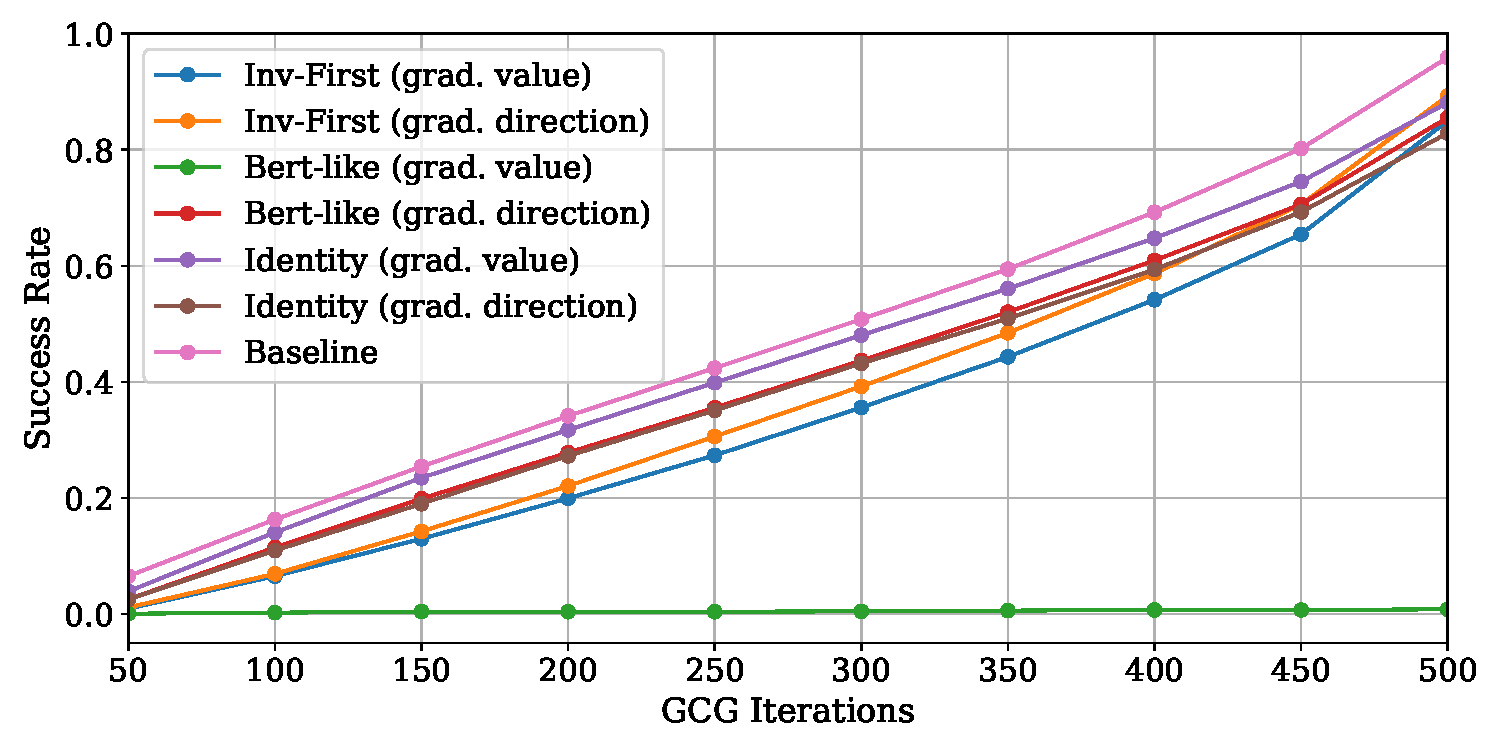
\includegraphics[width=0.9\linewidth]{assets/robustness/gcg_success_rate_varying_steps.pdf}
    \caption{GCG Success Rate varying according to the number of iterations performed}
    \label{fig:gcg_success_rate_varying_steps}
\end{figure}

In our experiments, we also studied the correlation between the number of GCG algorithm maximum allowed iterations and the success rate of the attack, always computed as the number of tokens that match between the LLM's responses to the original input $\bx$ and the attack input $\bx'$, while keeping all other hyperparameters, like the search window width, unaltered.
Interestingly, in \cref{fig:gcg_success_rate_varying_steps} some lines actually cross each other when increasing the number of GCG iterations: this may indicate that some variants are more effective at different values of the GCG iterations. For instance, \emph{Inv-First (grad. direction)}, represented as the orange line, is better than \emph{Bert-like (grad. direction)}, represented as the red line, when the number of allowed iterations is pretty low; however, at the end of the plot, at the maximum number of iterations tested, their effectiveness is the opposite. That being said, this phenomenon is not dramatic and makes only slight changes in the final results reported in the previously discussed table.

To have a better understanding of the GCG results listed in \cref{tab:small_tinystories_ce_attack},
we measured the following other metrics, always considering the subset of successful GCG attacks:
\begin{itemize}
    \item \emph{Original X CE-loss} is the $\loss_\text{CE}(f_\theta(\bx_0, ..., \bx_N); \by_0, ..., \by_M)$ - lower is better, since this means that $\by$ is a natural continuation of $\bx$ according to the model
    \item \emph{Attack X' CE-loss} is the $\loss_\text{CE}(f_\theta(\bx'_0, ..., \bx'_N); \by_0, ..., \by_M)$ - higher is better, since a low value means that $\by$ is a natural continuation of $\bx'$ according to the model, which is exactly the issue what we aim to solve
    \item \emph{Delta X CE-Loss} is the delta between the original prefix loss and the successful attack prefix found - the lower it is, the worst the attack was, so the more robust the model is when the attack is successful, since this is given as $\loss_\text{CE}(f_\theta(\bx)) - \loss_\text{CE}(f_\theta(\bx'))$ (as in the introduction in \cref{tab:evil_twins_examples}, the attack prefix has a lower loss than the natural sentence)
    \item \emph{KL-divergence} is the divergence between the probability distributions of the logits that correspond to the prediction of $\by$ and $\by'$; we want to measure how different are the logits, and thus the probability distributions of the next token: $KL(f_\theta(\bx_0, ..., \bx_N), f_\theta(\bx'_0, ..., \bx'_N))$
\end{itemize}
In all previous mathematical formulation, note that $f_\theta(\bx_0, ..., \bx_N)$ is the function which incorporates the LLM under attack and returns the logits that correspond to the prediction of the $\by$ output, not the ones that predict parts of the input prompt $\bx$ itself, as it would be wrong to consider for our analysis.

From the metrics in \cref{tab:small_tinystories_ce_attack}, we observe that robust variants, such as \emph{Identity (grad. direction)}, not only exhibit a substantially lower attack success rate (ASR) compared to the baseline, but also display a smaller increase in Cross-Entropy loss when the attack succeeds.
Recall that this \emph{delta} quantifies the extent to which the model is ``fooled'' by the attack, defined as the difference between the loss on the original, human-readable input and the loss on the adversarially generated sequence.
A higher delta indicates greater susceptibility, as the model interprets the attack sequence as being more strongly aligned with the target continuation $\by$.
Finally, the \textbf{KL-divergence} allows us to observe how much the output distributions returned by the LLM differ between $\bx$ and $\bx'$. The more different they are, the better the model can discriminate between them, recognizing that they are actually two distinct and different pieces of input.

\begin{table}[htbp]
\resizebox{\linewidth}{!}{
\begin{tabular}{rlcccc}
\toprule
           & \textbf{Grad.} & \textbf{Original X} & \textbf{Attack X'} & \textbf{Delta}     & \textbf{KL}           \\
           &                & \textbf{CE-loss ↓}  & \textbf{CE-loss}   & \textbf{CE-loss ↓} & \textbf{Divergence ↑} \\
\midrule
Baseline   &                & 13.28               & 10.97              & 2.31               & 2.19                  \\
\midrule
Identity   &                & 12.77               & 11.21              & 1.56               & 2.23                  \\
Bert-like  & Val.           & 13.26               & 10.25              & 3.01               & \textbf{54.19}        \\
Inv-First  &                & \textbf{11.09}      & 9.72               & \underline{1.37}   & 2.44                  \\
\midrule
Identity   &                & 12.58               & 11.12              & 1.46               & 2.47                  \\
Bert-like  & Dir.           & 11.49               & 10.34              & \textbf{1.15}      & 2.23                  \\
Inv-First  &                & \underline{11.21}   & 9.81               & 1.40               & 2.44                  \\
\bottomrule
\end{tabular}
}
\vspace{0.25cm}
\caption{Evaluation of the attack input prefix and the target model alone}
\label{tab:small_tinystories_ce_attack}
\end{table}

To have a complete evaluation, we adopt a similar approach to the one we used during inversion:
using a third-party model to compute some other statistics lets us abstract away from the biases in our LLMs.
Here, since the perplexity of the attack prefix is computed with a third-party independent model, it can easily return the real naturalness of the generated prefix, instead of being influenced by the attack itself and wrongly reporting that it will be even more natural than the human prefix.
Remember that we are considering only the successful attacks, ignoring the ones that have failed, since they are not useful to understand the quality of the attacks. Also, because of that, the results involving the \texttt{bert-like} variant using gradients as values will have a much smaller number of samples that participate in these metrics.

\begin{table}[htbp]
\centering
\begin{tabular}{rlccc}
\toprule
           & \textbf{Grad.} & \textbf{Original X} & \textbf{Attack X'}    & \textbf{Semantic}     \\
           &                & \textbf{Perplexity} & \textbf{Perplexity ↓} & \textbf{Similarity ↑} \\
\midrule
Baseline   &                & 44.14               & 17344.04              & 0.13                  \\
\midrule
Identity   &                & 43.98               & \textbf{8322.25}      & \textbf{0.18}         \\
Bert-like  & Val.           & 40.37               & 11817.21              & 0.11                  \\
Inv-First  &                & 44.81               & \underline{9431.09}   & \underline{0.16}      \\
\midrule
Identity   &                & 44.71               & 10929.21              & 0.15                  \\
Bert-like  & Dir.           & 44.74               & 10611.09              & 0.13                  \\
Inv-First  &                & 43.50               & 12344.85              & 0.13                  \\
\bottomrule
\end{tabular}
\vspace{0.25cm}
\caption{Evaluation of the attack input prefix and a third-party model}
\label{tab:small_tinystories_ce_attack_third_party}
\end{table}

\FloatBarrier{}
\subsection{Illustration of some adversarial samples}
In the following tables, we can observe some examples of the attack strings found by applying the GCG algorithm on the tested model variants,
as a mere qualitative illustration of the results we got.
Although they do not show attack strings that carry out the meaning of a $\by$ continuation, and they are still meaningless,
our training procedure allowed us to have a more robust model, since the attack success rate is lower in all the variants; some having a better result than others, but all of them in some way beat the baseline.


\begin{table}[htbp]
\centering
\footnotesize
\begin{tabularx}{\linewidth}{lXXc}\toprule
 & \textbf{Input} & \textbf{Output $\by$} & \textbf{Loss} \\
\midrule
$\bx$~: & cry. He wished he had listened to his mom. He stared at the earth and hoped someone would & \multirow{3}{*}{ help him. Suddenly, he heard a voice }  & 11.55 \\
$\bxa$: & Boboach att ag ChS asked cake.vel near pftautautue. thoughtautaut smart would & &  \textbf{ 10.11 } \\
%
\midrule
$\bx$~: & long time, ever since the house was abandoned. I have many stories to tell & \multirow{3}{*}{ you. Would you like to hear them? }  & 17.22 \\
$\bxa$: & gga,Dveryng Do magic belie the theationationicy black name never sayirt$<$unk$>$ & &  \textbf{ 12.99 } \\
%
% \midrule
% $\bx$~: & reat-grandpa. He was a brave explorer. He wore me on his & \multirow{3}{*}{ adventures. "Lily was amazed. She wanted to }  & 19.81 \\
% $\bxa$: & keyv L cakeeredirthday park play each eachv sail this others favoriteDet's favorite enjoyedet's & &  \textbf{ 17.86 } \\
\bottomrule
\end{tabularx}
\vspace{0.25cm}
\caption{Original inputs $\bx$ and adversarial examples $\bxa$ generated attacking with GCG the \texttt{Baseline} model.}
\end{table}


\begin{table}[htbp]
\centering
\footnotesize
\begin{tabularx}{\linewidth}{lXXc}\toprule
 & \textbf{Input} & \textbf{Output $\by$} & \textbf{Loss} \\
%
\midrule
$\bx$~: & Lily and Ben were friends who liked to play outside. But they did not like the same things. Lily & \multirow{3}{*}{ liked to make snowmen and snow angel }  & 13.22 \\
$\bxa$: & Lucy. Speez herself angO piecle you."lly named nexird opened cake".o.ter carrotmy & &  \textbf{ 12.14 } \\
%
\midrule
$\bx$~: & the ducks and the swings," Sam said." OK, Sam. That sounds fun," & \multirow{2}{*}{ Lily said.They opened the door and ste }  & 17.06 \\
$\bxa$: & Mommy than They TIon. up.Cleaseily am castle omisent. asked. crabo." & &  \textbf{ 13.85 } \\
%
\bottomrule
\end{tabularx}
\vspace{0.25cm}
\caption{Original inputs $\bx$ and adversarial examples $\bxa$ generated attacking with GCG the \texttt{Identity (grad. value)} model.}
\end{table}

\begin{table}[htbp]
\centering
\footnotesize
\begin{tabularx}{\linewidth}{lXXc}\toprule
 & \textbf{Input} & \textbf{Output $\by$} & \textbf{Loss} \\
%
\midrule
$\bx$~: & Lily and Ben were twins who liked to go on tours with their mom and dad. They & \multirow{3}{*}{ saw many new things and learned a lot. But }  & 24.14 \\
$\bxa$: & K forgot Tomriend rot became want or<unk><unk><unk> Onceriend sky. butterXgetherby & &  \textbf{ 23.08 } \\
%
\midrule
$\bx$~: & read books or draw pictures. They wanted to go outside and have fun. They looked at each other and & \multirow{3}{*}{ had an idea."Mom, we need to }  & 18.80 \\
$\bxa$: & Lis conizz Maskock!" t angry had nois What oyM sleep Benirdixfe & &  \textbf{ 18.27 } \\
%
\bottomrule
\end{tabularx}
\vspace{0.25cm}
\caption{Original inputs $\bx$ and adversarial examples $\bxa$ generated attacking with GCG the \texttt{Bert-like (grad. value)} model.}
\end{table}

\begin{table}[htbp]
\centering
\footnotesize
\begin{tabularx}{\linewidth}{lXXc}\toprule
 & \textbf{Input} & \textbf{Output $\by$} & \textbf{Loss} \\
%
\midrule
$\bx$~: & Lila and Ben were adventurous kids. They liked to explore new places and try new things. & \multirow{3}{*}{ One day, they went to the beach with their mom }  & 18.64 \\
$\bxa$: & so rest come so an One rock o per who<s> fr balling, M cars Whisk listen. likes Spot. & &  \textbf{ 13.47 } \\
%
\midrule
$\bx$~: & One day, a little boy named Tim found a peanut on the ground. He picked it up and & \multirow{3}{*}{ showed it to his mom. "Mom, what is this?" }  & 19.36 \\
$\bxa$: & pudd likesnn.hing It Sara "It where M whereanc It where pen where some?" madei & &  \textbf{ 17.06 } \\
%
\bottomrule
\end{tabularx}
\vspace{0.25cm}
\caption{Original inputs $\bx$ and adversarial examples $\bxa$ generated attacking with GCG the \texttt{Inv-First (grad. value)} model.}
\end{table}


\begin{table}[htbp]
\centering
\footnotesize
\begin{tabularx}{\linewidth}{lXXc}\toprule
 & \textbf{Input} & \textbf{Output $\by$} & \textbf{Loss} \\
%
\midrule
$\bx$~: & ." She is happy. She made a new pattern.She moves on to the flowers. & \multirow{3}{*}{ She says, "One, two, three, f }  & 11.15 \\
$\bxa$: & e Sheleix ey,se, amix4$<$unk$>$t. says, Herix help, in pawixt. & &  \textbf{ 9.55 } \\
%
\midrule
$\bx$~: & Imagine standing in a park with many trees and a big green lawn. & \multirow{3}{*}{ In the middle of the park is }  & 16.43 \\
$\bxa$: & fere re'age  att ApenXapard. thankarn vo park.XX keyft park. & &  \textbf{ 11.73 } \\
%
\bottomrule
\end{tabularx}
\vspace{0.25cm}
\caption{Original inputs $\bx$ and adversarial examples $\bxa$ generated attacking with GCG the \texttt{Identity (grad. direction)} model.}
\end{table}

\begin{table}[htbp]
\centering
\footnotesize
\begin{tabularx}{\linewidth}{lXXc}\toprule
 & \textbf{Input} & \textbf{Output $\by$} & \textbf{Loss} \\
%
\midrule
$\bx$~: & of plastic and has perfume on it. It does not grow or need water. It is & \multirow{3}{*}{ not real."Lily was confused and }  & 18.72 \\
$\bxa$: & everything her small, from pus Tim ThatF$<$unk$>$ LV paper I h listen LI with. do & &  \textbf{ 15.15 } \\
%
\midrule
$\bx$~: & reat-grandpa. He was a brave explorer. He wore me on his & \multirow{3}{*}{ adventures."Lily was amazed. She wanted to }  & 20.26 \\
$\bxa$: & by ta anotherizCcessious rcessly, Lious tower her ask derirthdayI its & &  \textbf{ 17.54 } \\
%
\bottomrule
\end{tabularx}
\vspace{0.25cm}
\caption{Original inputs $\bx$ and adversarial examples $\bxa$ generated attacking with GCG the \texttt{Bert-like (grad. direction)} model.}
\end{table}

\begin{table}[htbp]
\centering
\footnotesize
\begin{tabularx}{\linewidth}{lXXc}\toprule
 & \textbf{Input} & \textbf{Output $\by$} & \textbf{Loss} \\
%
\midrule
$\bx$~: & Ben and Sam were friends who liked to play with toys. They had many toys, but their favorite was a & \multirow{3}{*}{ helicopter. The helicopter }  & 13.76 \\
$\bxa$: & p nodd nodd clotZub fam Do un said,ball wr." hitac bi'reide.-x & &  \textbf{ 11.14 } \\
%
\midrule
$\bx$~: & Lily was excited to go to school. She liked to learn new things from her teach. She also & \multirow{3}{*}{ liked to play with her friends. Today, they }  & 17.10 \\
$\bxa$: & its botindbbougower. seenhere eezick moral food Gra peop everyoun'oun ever & &  \textbf{ 16.34 } \\
%
\bottomrule
\end{tabularx}
\vspace{0.25cm}
\caption{Original inputs $\bx$ and adversarial examples $\bxa$ generated attacking with GCG the \texttt{Inv-First (grad. direction)} model.}
\end{table}


\FloatBarrier{}
\section{Forward LM Evaluation}
Finally, we tested that these models are still functioning properly in forward mode, without experiencing \textbf{performance degradation}. Checking out the perplexity during training and validation, it has been observed that the performance of the custom models with the regularization term on the gradients $\nabla_\be\loss_\text{CE}$ does not penalize the model's ability to speak fluently during standard usage in forward mode. This is not obvious, since many times in Adversarial Training in literature, the model may require many more parameters and training time to reach the same final objective, since part of the model capacity will be used by the adversarial training procedure, whatever it is in general.
In \cref{tab:inverse_lm__forward_mode_quantitative} we can observe that the worst model is \emph{Inv-First (grad. value)}.
This relatively high perplexity value is also confirmed in the qualitative examples in the tables below, where the sentences are by far the ones that make less sense and seem more confused and repetitive.


\begin{table}[htbp]
\vspace{0.5cm}
\centering
\begin{tabular}{rlcc}
\toprule
           & \textbf{Grad.} & \textbf{Perplexity ↓} & \textbf{CE Loss ↓} \\
\midrule
Baseline   &                & \textbf{4.83}         & \textbf{1.58}      \\
\midrule
Identity   &                & \underline{5.07}      & \underline{1.63}   \\
Bert-like  & Val.           & 5.79                  & 1.76               \\
Inv-First  &                & 8.41                  & 2.13               \\
\midrule
Identity   &                & \underline{5.08}      & \underline{1.62}   \\
Bert-like  & Dir.           & 5.42                  & 1.69               \\
Inv-First  &                & 6.82                  & 1.92               \\
\bottomrule
\end{tabular}
\vspace{0.25cm}
\caption{Quantitative forward mode evaluation}
\label{tab:inverse_lm__forward_mode_quantitative}
\end{table}


\begin{table}[htbp]
\footnotesize
\begin{NiceTabular}{rl|[tikz=dotted]X}
\toprule
           & \textbf{Grad.} & \textbf{Completion for ``One day,''} \\
\midrule
Baseline   &                & a little boy named Tim wanted to travel to a far mountain. He asked his dad for a raft, \\
\midrule
Identity   &                & a little girl named Lucy went to the park with her mom. Lucy liked to play on the swings \\
Bert-like  & Val.           & a little boy was walking in the park. He noticed a big, shiny object in the park. \\
Inv-First  &                & they pinch. They find gold. They take pictures of stars. \\
\midrule
Identity   &                & a little girl named Amy was playing outside. She saw a big tree and thought it was a toy. \\
Bert-like  & Dir.           & a little girl named Lucy was playing in the garden. She saw a shiny ring on a branch. \\
Inv-First  &                & hey went to the beach with his mom. He saw something shiny and strange inside. \\
\bottomrule
\end{NiceTabular}

\vspace{1cm}

\begin{NiceTabular}{rl|[tikz=dotted]X}
\toprule
           & \textbf{Grad.} & \textbf{Completion for ``Once there was a''} \\
\midrule
Baseline   &                & little girl called Emma. She was 3 years old and she liked to explore new places. Everywhere she went, she saw something special. \\
\midrule
Identity   &                & boy who was very enthusiastic. Every day he would go outside and go out and play in the sun \\
Bert-like  & Val.           & girl who loved to play. One day she decided to go on a walk in her neighbourhood. \\
Inv-First  &                & learn to others, but she also learn something new things she should not have shared with others. \\
\midrule
Identity   &                & little boy who was very curious. He wanted to know why he was so interesting. He decided to explore the world around him. \\
Bert-like  & Dir.           & small girl named Mary. Mary was only three years old and she loved to explore the world. \\
Inv-First  &                & girl named Sarah. She was very curious. She wanted to see what was in her room. \\
\bottomrule
\end{NiceTabular}
\vspace{0.25cm}
\caption{Example completions for the given prompt, in forward mode}
\label{tab:inverse_lm__forward_mode_execution}
\end{table}





\subbib{}
\end{document}